\section{Research}%
\label{sec:research}

\emph{This section contains literature research that applies to the SHARP-PS project. The workings of fuel cells are explained in detail. A comparison is made that evaluates the effectiveness of energy storage as hydrogen tanks versus batteries. Several papers are described of other projects that are similar to the SHARP project. The results and design choices made during these projects might be of interest during the SHARP-PS project.}

\subsection{PEM Fuel Cells}
Fuel cells are a technology that produce electricity from gases directly without combustion. There are many different types of fuel cells that run on different types of gases. These include solid oxide fuel cells (SOFC), direct methanol fuel cells (DMFC) and proton exchange membrane fuel cells (PEMFC). The PEMFC is used widely as it has a relatively high power density and a low operating temperature \cite{Kim:NaBH}. These properties are especially beneficial for UAV power systems.

The book \emph{Fuel Cells} by \citeA{revankar-2016} describes the working of the PEMFC in great detail. The PEMFC works by letting hydrogen undergo a series of electrochemical reactions. At the anode the hydrogen is split into protons ($H^+$) and electrons ($e^-$). The protons pass through the Proton Exchange Membrane (PEM), but the electrons can't pass through this membrane and must follow the external electrical circuit. The protons and electrons both arrive at the cathode where they react with oxygen to form water. This process is shown in a schematic diagram in figure~\ref{fig:fuelcell single}.

% Introduce Stack?
As a single fuel cell typically produces 0.7 volts, multiple cells are often connected in a stack. The membrane electrode assembly (MEA) is sandwiched between two conducting plates that have integrated flow channels for the hydrogen, oxygen and water. A schematic overview of a stack including three cells is provided in figure~\ref{fig:fuelcell stack}.

\begin{figure}[htp]
    \begin{subfigure}{0.5\textwidth}
        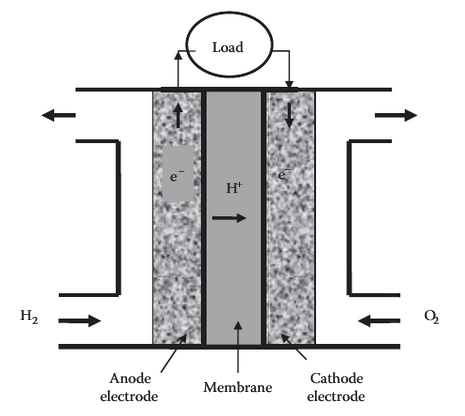
\includegraphics[width=0.9\linewidth, height=8cm]{media/FuelCell.png}
        \caption{Single Fuel Cell}
        \label{fig:fuelcell single}
    \end{subfigure}
    \begin{subfigure}{0.5\textwidth}
        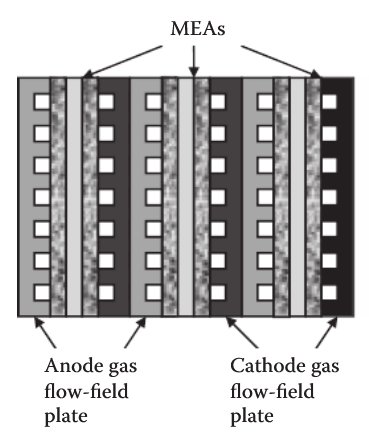
\includegraphics[width=0.9\linewidth, height=7cm]{media/FuelCellStack.png}
        \caption{Fuel Cell Stack}
        \label{fig:fuelcell stack}
    \end{subfigure}
    \caption{Fuel Cell Schematic Diagrams}
    \label{fig:fuelcell overview}
\end{figure}

As visible in figure~\ref{fig:fuelcell single}, hydrogen not only flows into the anode side of the fuel cell, but also out of that side. Simply leaving this side open to the air not only wastes a lot of unused hydrogen but also poses a major safety risk~\cite{Li:circulation}. If this side of the anode is simply blocked off, impurities in the hydrogen and liquid water generated by the reaction accumulate over time, blocking the hydrogen supply. Instead, a purge valve can be installed that periodically purges the anode side and removes gas impurities and excess water. While this design is simple it still leads to periodic voltage drops and reduced power output.
\citeauthor{Li:circulation} introduces several circulation mechanisms to prevent this and enhance both safety and fuel utilisation. These circulation mechanisms include recirculation pumps, ejector valves or a combination of both. However both of these systems only become efficient for fuel cells operating above 80 kW, which is orders of magnitude higher than required for the fuel cell in this project.

\subsection{Comparison of Energy Storage Methods}
The SHARP project aims to extend the flight time of drones and possibly small aircraft in the future. It aims to do this by providing an alternative energy source that is more weight efficient than current solutions. To keep track of the progress and improvements that are made by the SHARP project the energy density of current solutions are analysed.

Different aspects of energy density play a role in aviation systems. Most important is the gravimetric energy density, which refers to the amount of stored energy per unit mass. For hydrogen this is 142 MJ/kg, nearly three times that of kerosene at 50 MJ/kg. However, volumetric energy density also plays a role and it refers to the amount of stored energy per unit volume. For hydrogen at atmospheric pressure this is only 0.01 MJ/L while for kerosene this is much higher at 35 MJ/L. For this reason, hydrogen is often stored in pressurised tanks or as a cryogenic liquid. This significantly increases the volumetric energy density as can be seen in table~\ref{tab:fuels}.

\begin{table}[htp]
    \centering
    \begin{tabularx}{0.75\textwidth}{X r r}
        \toprule
        \textbf{Fuel}      & \textbf{Gravimetric [MJ/kg]} & \textbf{Volumetric [MJ/L]} \\
        \midrule
        Gasoline           & 46                           & 34                         \\
        Kerosene           & 50                           & 35                         \\
        Hydrogen (1 bar)   & 142                          & 0.01                       \\
        Hydrogen (350 bar) & 142                          & 3                          \\
        Hydrogen (700 bar) & 142                          & 5                          \\
        Hydrogen (liquid)  & 142                          & 8.5                        \\
        \bottomrule
    \end{tabularx}
    \caption{Energy density of fuels}
    \label{tab:fuels}
\end{table}

The gravimetric energy density of hydrogen itself may be very high, however pressurised storage vessels are quite heavy and thus their weight cannot be neglected. Generally, the hydrogen stored in a pressurised cylinder only contributes 2 to 5\% of the total weight of the cylinder. This weight percentage is dependant on the cylinder shape and size. Intelligent Energy, a fuel cell supplier, has provided an overview of currently available hydrogen storage cylinders of different sizes from different suppliers~\cite{IE:cylinders}. This is shown in figure~\ref{fig:IE cylinders}.

\begin{figure}[htp]
    \centering
    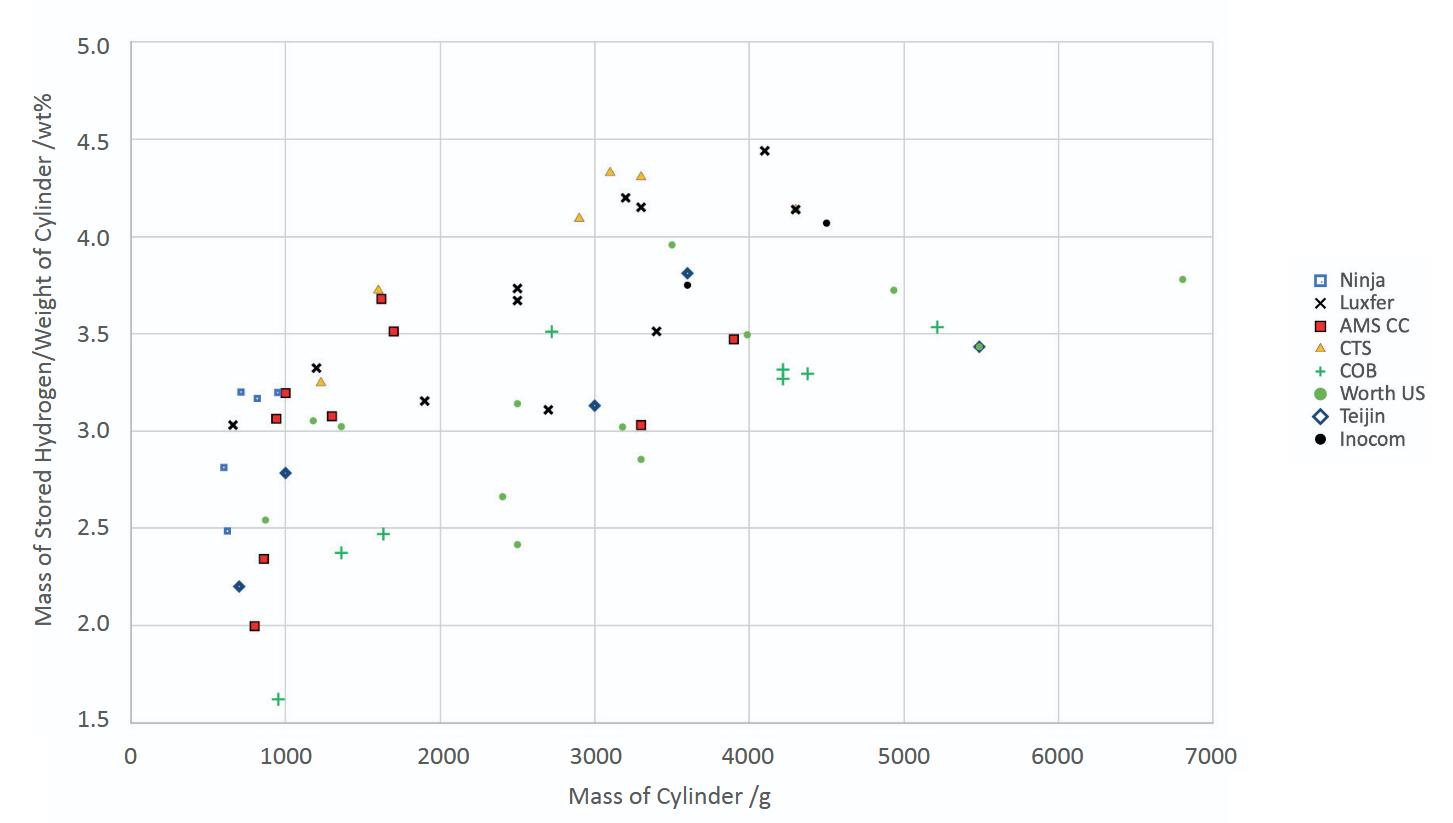
\includegraphics[width=0.75\textwidth]{media/IE_cylinders.png}

    \caption{Gravimetric Energy Density comparison of hydrogen Cylinders by Intelligent Energy}
    \label{fig:IE cylinders}
\end{figure}

Hydrogen cylinders can now be compared with LiPo batteries, which are a popular energy storage solution for UAVs. From figure~\ref{fig:IE cylinders} it is clear that hydrogen cylinders become more weight efficient at larger sizes. LiPo batteries also come in different shapes and sizes, however they do not share this increase in efficiency with hydrogen cylinders. A comparison has been made the energy density of different systems at different storage sizes, this is shown in figure~\ref{fig:Energy Storage}. The comparison includes some of the smaller Hydrogen cylinders from AMS CC from the comparison by Intelligent Energy, as well as some even smaller hydrogen tanks by MyH2. Several LiPo batteries have been included as well as batteries of some popular drones by DJI. A fuel cell efficiency of 40\% was assumed when determining the energy capacity of the hydrogen cylinders.

\begin{figure}[htp]
    \centering
    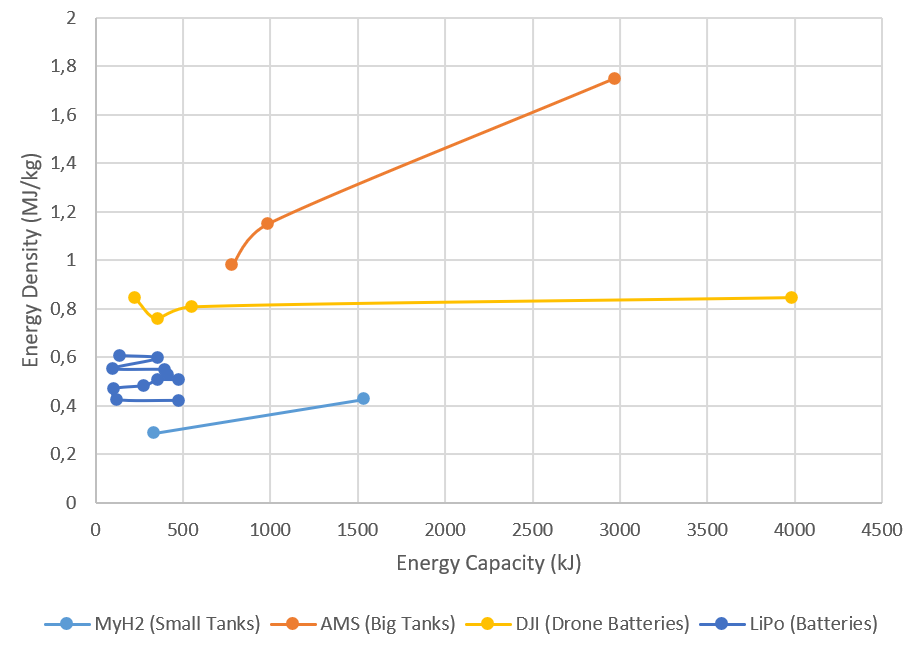
\includegraphics[width=0.75\textwidth]{media/Energy_Storage.png}
    \caption{Gravimetric Energy Density comparison of different energy storage solutions}
    \label{fig:Energy Storage}
\end{figure}

The goal of this comparison is to find a break-even point where hydrogen cylinders become more efficient than batteries. Unfortunately, figure~\ref{fig:Energy Storage} does not give an exact point, however the first hydrogen cylinder that is more efficient than batteries has an energy capacity of 780 kJ, above this point hydrogen cylinders are more efficient than batteries. Noteworthy is that this is more than double the capacity of the DJI Inspire, a large consumer drone, at 350 kJ. This means that for doubling the flight time of this drone, it would require less mass to just add an extra battery than to replace its battery with a hydrogen system.

Figure~\ref{fig:Energy Storage} compares the gravimetric energy density of energy storage solutions,  but ignores the weight of the system required to actually retrieve this energy. Figure~\ref{fig:Energy Storage} was made specifically for the context of the SHARP project where hydrogen is generated at a using a CGG. In order to decouple the constant rate of energy generation from the fluctuating energy consumption of the drone an energy buffer is required. Figure~\ref{fig:Energy Storage} allows comparison for using a battery or hydrogen cylinder as this buffer. In this specific case, the fuel cell system is required regardless of whether the energy buffer is implemented as a battery or as a hydrogen tank, and thus its weight does not play a role in their comparison.

However, when comparing using hydrogen cylinders with a fuel cell to using batteries without a fuel cell, the weight of the fuel cell must also be considered.



\subsection{Hydrogen Drones}
Several studies have been performed on the feasibility of hydrogen drones using PEMFCs. One notable example is \citeA{NLR:HYDRA}, their HYDRA project produced an 8kg hexacopter running on an 800W fuel cell for the Royal Netherlands Aerospace Centre (NLR). Their HYDRA-1B power system achieved and energy density of about 0.36 kWh/kg which is higher than that of commercial LiPo batteries at about 0.2 kWh/kg and still has significant potential for improvement. Their paper on the HYDRA project goes into detail about the drone design and part selection as well as hydrogen safety. This may provide a starting point for the design of the SHARP-PS project as the target scale of the drone and power system are similar.

Another example is \citeA{Nederdrone} who produced a Vertical Take-Off and Landing (VTOL) UAV called the Nederdrone, which runs on the same 800W fuel cell. In addition to stating the processes of fuel cell selection and drone design, they also go into detail about their hybrid power system using batteries to supply additional power during peak load.

Notable is that both systems use the same fuel cell by Intelligent Energy in combination with backup batteries. In addition to that, both projects are recent projects executed in the Netherlands, which may enable easy consultation if necessary. Stellar Space Industries has contacted NLR, who have expressed interest in the SHARP project.

\newpage

